\documentclass[a4paper,10pt, DIV10]{scrartcl}

\usepackage[ngerman]{babel}
\usepackage[T1]{fontenc}
\usepackage[ansinew]{inputenc}
\usepackage{graphicx}
\usepackage{multicol}
\usepackage{float}
\usepackage{amsmath}
\usepackage{dsfont}
\usepackage{listings}
\usepackage{lastpage}
\usepackage{scrpage2}
\usepackage{url}

\ihead{VirtualBox und POTATOES Installationsanleitung}
\cfoot{Seite \thepage~von \pageref{LastPage}}
\ofoot{\today}
\setheadsepline{1pt}
\setfootsepline{0.5pt}
\pagestyle{scrheadings}
\usepackage{setspace}
\onehalfspacing
\setlength{\parindent}{0em}

\begin{document}

\begin{center}
Diese Anleitung ist gepr�ft f�r Sun VirtualBox 3.0.2
\end{center}

\section*{\underline {VirtualBox-Download:}}
\url{http://www.virtualbox.org/wiki/Downloads}

\url{http://www.virtualbox.org/wiki/Linux_Downloads}

\section*{\underline {VirtualBox-Installation:}}
\begin{enumerate}
	\item Ausf�hren der entsprechenden VirtualBox-Setupdatei
	
\textbf{Wichtig:} Wir empfehlen, die Frage nach der Installation des USB-Controllers, sowie des Netzwerkadapters und -dienstes
mit \textit{"`Ja"'} zu beantworten.
	\item VirtualBox starten
	\item Men�punkt: Datei -> Manager f�r virtuelle Medien
		\begin{center}
		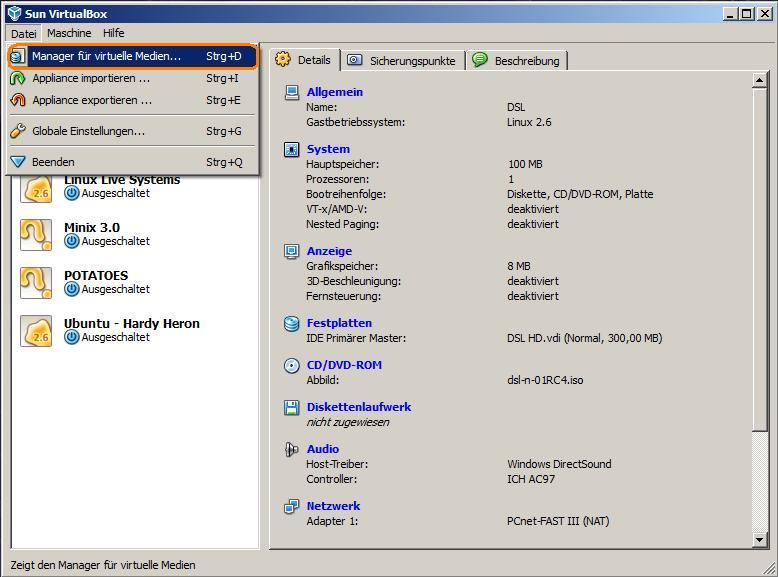
\includegraphics[width=0.75\textwidth]{Screen1.jpg}
		\end{center}
\pagebreak
\item Virtuelles Festplattenimage hinzuf�gen (Schritt I)
		\begin{center}
		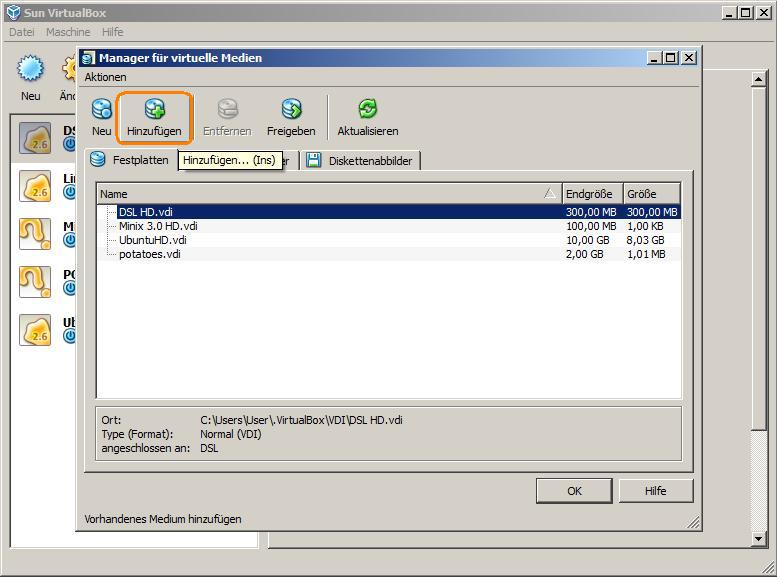
\includegraphics[width=0.75\textwidth]{Screen2.jpg}
		\end{center}

\item Virtuelles Festplattenimage hinzuf�gen (Schritt II)

\textbf{Wichtig:} Imagedatei befindet sich in der gepackten Datei \textit{POTAOES\_Xubuntu.zip}. Diese Datei in ein eigenes Verzeichnis auf der Festplatte extrahieren.
		\begin{center}
		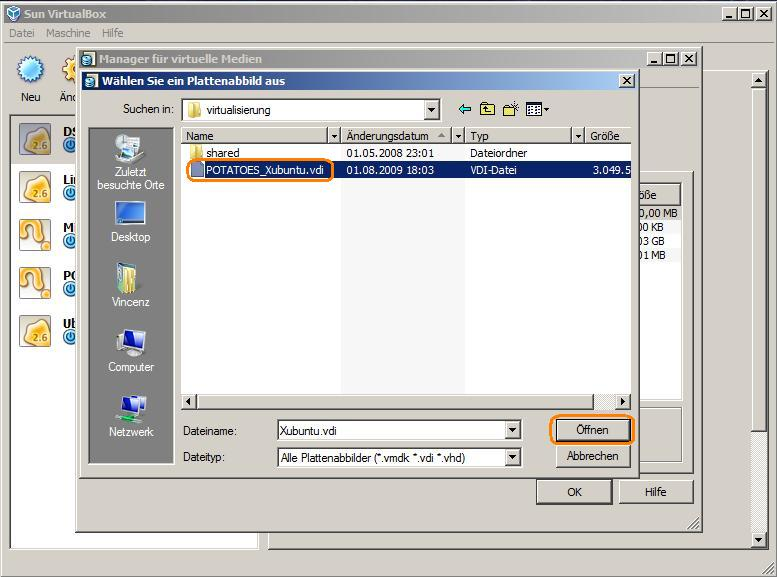
\includegraphics[width=0.75\textwidth]{Screen3.jpg}
		\end{center}
\pagebreak
\item Virtuelles Festplattenimage hinzuf�gen (Schritt III)
		\begin{center}
		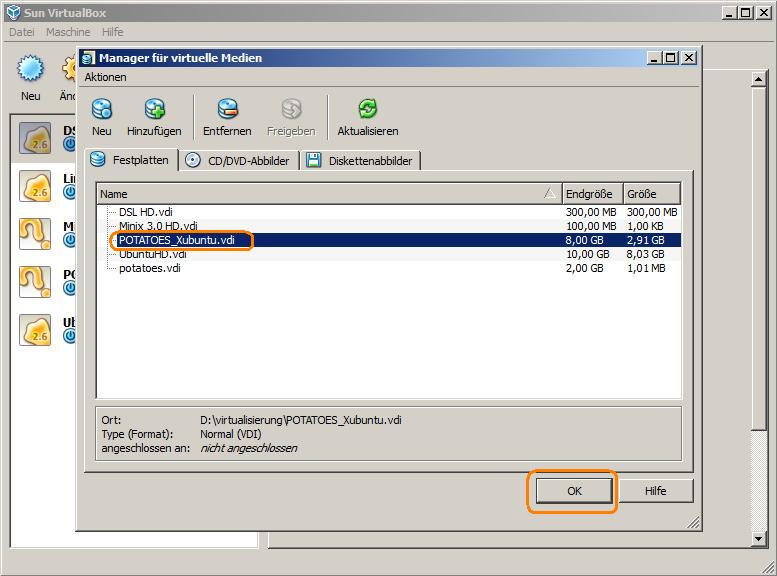
\includegraphics[width=0.75\textwidth]{Screen4.jpg}
		\end{center}

\item Virtuelle Maschine einrichten (Schritt I)
		\begin{center}
		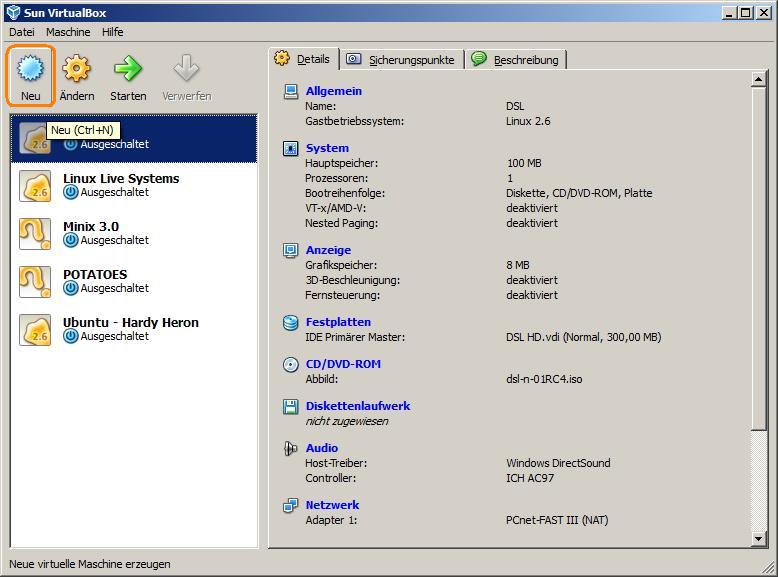
\includegraphics[width=0.75\textwidth]{Screen5.jpg}
		\end{center}
\pagebreak	
\item Virtuelle Maschine einrichten (Schritt II)
		\begin{center}
		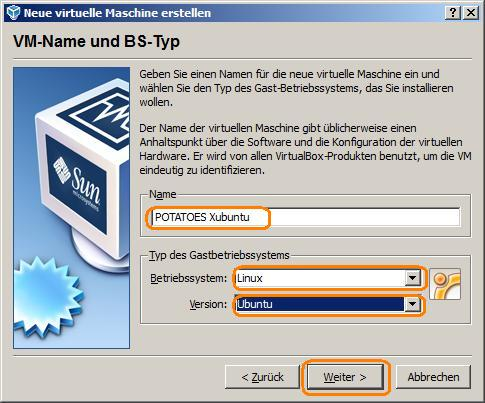
\includegraphics[width=0.75\textwidth]{Screen6.jpg}
		\end{center}
		
\item Virtuelle Maschine einrichten (Schritt III)
		\begin{center}
		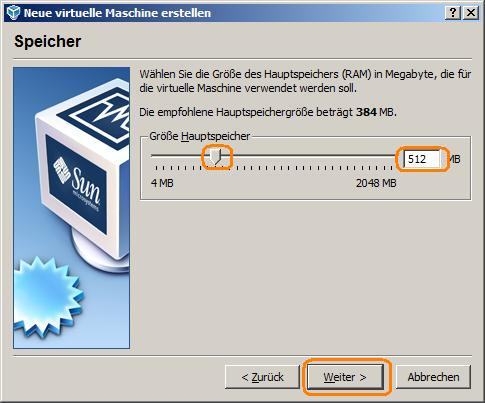
\includegraphics[width=0.75\textwidth]{Screen7.jpg}
		\end{center}
\pagebreak
\item Virtuelle Maschine einrichten (Schritt IV)

\textbf{Wichtig:} An dieser Stelle das vorher installierte Festplattenimage ausw�hlen.
		\begin{center}
		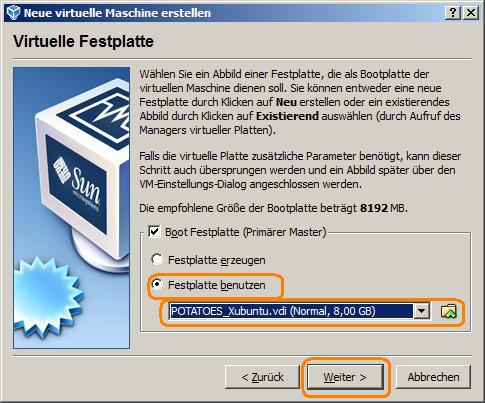
\includegraphics[width=0.75\textwidth]{Screen8.jpg}
		\end{center}

\item \textbf{(Optional)} Einstellungen der Virtuellen Maschine anpassen
		\begin{center}
		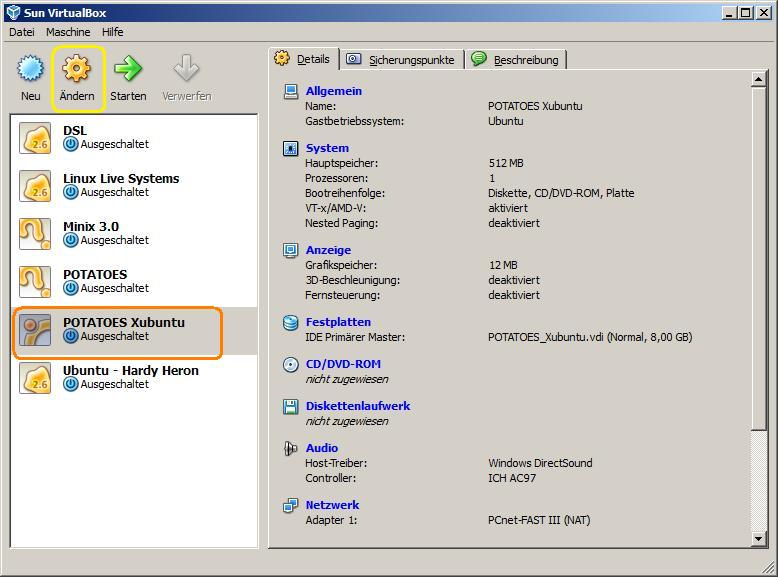
\includegraphics[width=0.75\textwidth]{Screen9.jpg}
		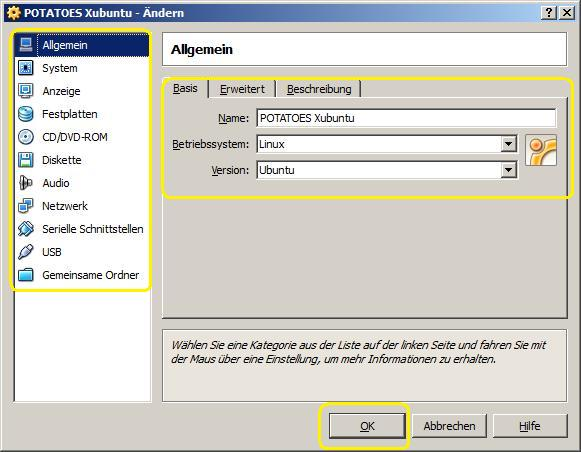
\includegraphics[width=0.75\textwidth]{Screen10.jpg}
		\end{center}

\item Virtuelle Maschine starten
		\begin{center}
		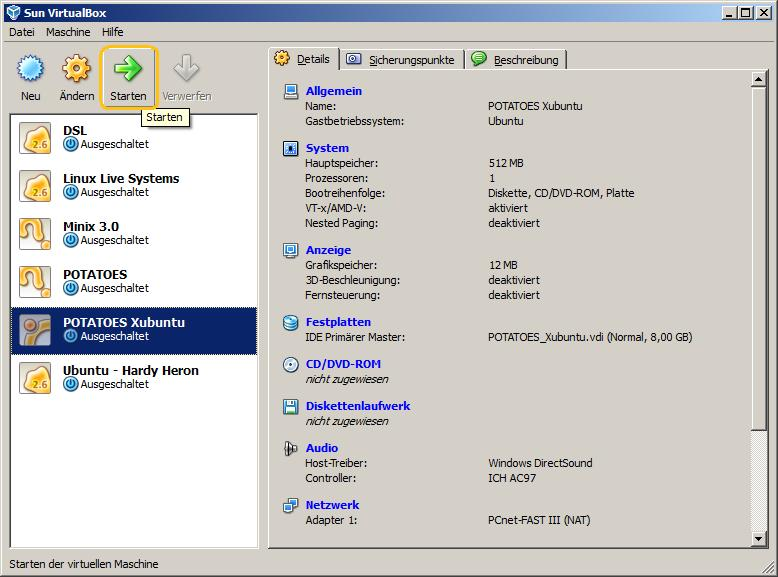
\includegraphics[width=0.75\textwidth]{Screen11.jpg}
		\end{center}
		
\pagebreak
\item Fertig

Nachdem die Virtuelle Maschine gebootet hat, kann die gew�nschte Bildschirmaufl�sung ausgew�hlt werden.
Die Desktopicons bieten folgende Funktionalit�t:
\begin{itemize}
\item \textbf{Build \& Run} - �bersetzt den Kernel und f�hrt das System virtualisiert aus.
\item \textbf{Eclipse} - Startet die vorkonfigurierte Entwicklungsumgebung
\item \textbf{Terminal} - �ffnet eine Terminalsession
\item \textbf{POTATOES folder} - �ffnet den Projektordner    
\end{itemize}
		\begin{center}
		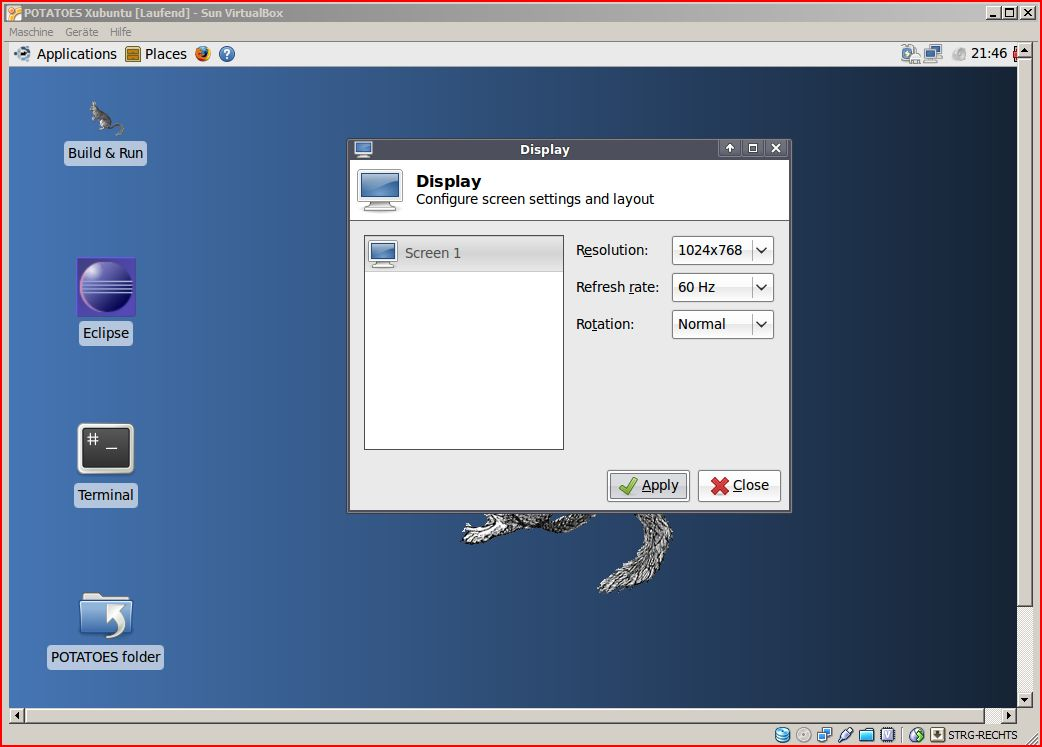
\includegraphics[width=0.75\textwidth]{Screen12.jpg}
		\end{center}
		
\end{enumerate}

\end{document}